\documentclass[10pt,notes,compress,aspectratio=169]{beamer}
\usepackage[brazil]{babel}  
\usepackage[utf8]{inputenc}
\usepackage[T1]{fontenc}

\usefonttheme[onlymath]{serif}
\usepackage{beamerthemesplit}
\usetheme{Antibes}

\beamersetuncovermixins{\opaqueness<1->{25}}{\opaqueness<2->{15}}
\setbeamertemplate{itemize items}[triangle]
\setbeamertemplate{enumerate item}{\insertenumlabel)}
\setbeamertemplate{enumerate subitem}{\insertenumlabel-\insertsubenumlabel)}
\setbeamertemplate{caption}[numbered]
\setbeamertemplate{mini frames}{}
\setbeamertemplate{navigation symbols}{}
\setbeamerfont{block title}{size=\scriptsize}
\setbeamerfont{frametitle}{size=\small}
\beamertemplatenavigationsymbolsempty

\newcommand{\hrefcolor}[2]{\textcolor{BlueGreen}{\href{#1}{#2}}}

% Rotating Objects and Captions
\usepackage{hvfloat}

\usepackage{natbib}
\usepackage[brazilian]{cleveref}
\crefname{lstlisting}{lista}{listas}
\Crefname{lstlisting}{Lista}{Listas}

% equation stuff
\usepackage{nicefrac}
%\usepackage{cancel}

% BEGIN - listings - code in LaTeX
\usepackage{listings}
\renewcommand\lstlistingname{Lista}
\lstset{
  language=octave,
  breaklines=true,
  postbreak=\mbox{$\hookrightarrow$\space},
  basicstyle=\linespread{1}\small\ttfamily,
  %numbers=left,
  numbers=none,
  %frame=lines,
  xleftmargin=0.5cm,
  frame=none,
  framexleftmargin=0.5em,
  framexrightmargin=0.5em,
  %backgroundcolor=\color{light-gray},
  showstringspaces=false,
  upquote=true,
  commentstyle=\color{gray},
  %morecomment=[f][\color{gray}][28]{\#},
  morecomment=[l]{\#\#},
  literate=%
           {á}{{\'a}}1
           {í}{{\'i}}1
           {é}{{\'e}}1
           {ú}{{\'u}}1
           {ó}{{\'o}}1
           {à}{{\`a}}1
           {ã}{{\~a}}1
           {õ}{{\~o}}1
           {â}{{\^a}}1
           {ê}{{\^e}}1
           {ô}{{\^o}}1
           {ç}{{\c{c}}}1
           {Á}{{\'A}}1
           {Í}{{\'I}}1
           {É}{{\'E}}1
           {Ú}{{\'U}}1
           {Ó}{{\'O}}1
           {À}{{\`A}}1
           {Ã}{{\~A}}1
           {Õ}{{\~O}}1
           {Â}{{\^A}}1
           {Ê}{{\^E}}1
           {Ô}{{\^O}}1
           {Ç}{{\c{C}}}1
}
% END - listings

\patchcmd{\theorem}{Theorem}{Teorema}{}{}
\patchcmd{\corollary}{Corollary}{Corolário}{}{}
\patchcmd{\lemma}{Lemma}{Lema}{}{}
\patchcmd{\proposition}{Proposition}{Proposição}{}{}
\patchcmd{\axiom}{Axiom}{Axioma}{}{}
\patchcmd{\example}{Example}{Exemplo}{}{}
\patchcmd{\definition}{Definition}{Definição}{}{}
\patchcmd{\remark}{Remark}{Observação}{}{}

\newcommand*{\theorembreak}{\usebeamertemplate{theorem end}\framebreak\usebeamertemplate{theorem begin}}
\newcommand*{\proofbreak}{\hfill ...\usebeamertemplate{proof end}\framebreak\usebeamertemplate{proof begin}{\scriptsize\color{gray}continuação...}\\}
\newcommand*{\examplebreak}{\hfill ...\usebeamertemplate{theorem end}\framebreak\usebeamertemplate{theorem begin}{\scriptsize\color{gray}continuação...}\\}
\newcommand*{\exercisebreak}{\hfill ...\usebeamertemplate{theorem end}\framebreak\usebeamertemplate{theorem begin}{\scriptsize\color{gray}continuação...}\\}
\newcommand*{\lemmabreak}{\hfill ...\usebeamertemplate{theorem end}\framebreak\usebeamertemplate{theorem begin}{\scriptsize\color{gray}continuação...}\\}
\newcommand*{\blockbreak}{\hfill ...\usebeamertemplate{block end}\framebreak\usebeamertemplate{block begin}{\scriptsize\color{gray}continuação...}\\}
\newcommand*{\definitionbreak}{\hfill ...\usebeamertemplate{theorem end}\framebreak\usebeamertemplate{theorem begin}{\scriptsize\color{gray}continuação...}\\}

% math symbols

% symbol for independet
\newcommand\independent{\protect\mathpalette{\protect\independenT}{\perp}}
\def\independenT#1#2{\mathrel{\rlap{$#1#2$}\mkern2mu{#1#2}}}
% Real Numbers
\newcommand\RealNumber{{\rm I\!R}}
% Expected value, Variance and Covariance
\newcommand{\E}{\mathrm{E}}
\newcommand{\Var}{\mathrm{Var}}
\newcommand{\Cov}{\mathrm{Cov}}

%%%%%%%%%%%%%%%%%
% math cancel to (down arrow)
\makeatletter
% #1, #2 offset of label   #6 extra width to clear arrowhead
% #3, #4 vector direction  #7 superscript label style
% #5 vector width          #8 superscript label
\def\cantox@vector#1#2#3#4#5#6#7#8{%
  \dimen@.5\p@
  \setbox\z@\vbox{\boxmaxdepth.5\p@
   \hbox{\kern-1.2\p@\kern#1\dimen@$#7{#8}\m@th$}}%
  \ifx\canto@fil\hidewidth  \wd\z@\z@ \else \kern-#6\unitlength \fi
  \ooalign{%
    \canto@fil$\m@th \CancelColor
    \vcenter{\hbox{\dimen@#6\unitlength \kern\dimen@
      \multiply\dimen@#4\divide\dimen@#3 \vrule\@depth\dimen@\@width\z@
      \vector(#3,-#4){#5}%
    }}_{\raise-#2\dimen@\copy\z@\kern-\scriptspace}$%
    \canto@fil \cr
    \hfil \box\@tempboxa \kern\wd\z@ \hfil \cr}}
\def\bcancelto#1#2{\let\canto@vector\cantox@vector\cancelto{#1}{#2}}
\makeatother
%%%%%%%%%%%%%%%%%


%%%%%%%%%%%%%%%%%
% left-right arrow
\makeatletter
\newcommand\xleftrightarrow[2][]{%
  \ext@arrow 9999{\longleftrightarrowfill@}{#1}{#2}}
\newcommand\longleftrightarrowfill@{%
  \arrowfill@\leftarrow\relbar\rightarrow}
\makeatother
%%%%%%%%%%%%%%%%%


%%%%%%%%%%%%%%%%%
% commands to resume enumeration across frames 
\newcounter{sauvegardeenumi}
\newcommand{\asuivre}{\setcounter{sauvegardeenumi}{\theenumi}}
\newcommand{\suite}{\setcounter{enumi}{\thesauvegardeenumi}}
%%%%%%%%%%%%%%%%%

%%%%%%%%%%%%%%%%% underbrase - font size no change
\newcommand*{\KeepStyleUnderBrace}[1]{%
  \mathop{%
    \mathchoice
    {\underbrace{\displaystyle#1}}%
    {\underbrace{\textstyle#1}}%
    {\underbrace{\scriptstyle#1}}%
    {\underbrace{\scriptscriptstyle#1}}%
  }\limits
}
%%%%%%%%%%%%%%%%%

%%%%%%%%%%%%%%%%% math operators
\DeclareMathOperator*{\argmin}{\arg\!\min}
\DeclareMathOperator*{\argmax}{\arg\!\max}
\DeclareMathOperator{\sign}{sign}
\DeclareMathOperator{\Tr}{Tr}
%%%%%%%%%%%%%%%%%


\title[Teoria da Informação]{Teoria da Informação}
\author[Prof. Leonardo Araújo]{Prof. Leonardo Araújo}
\date{}

\begin{document}
\frame{\titlepage}

\frame{\centering 
\includegraphics[width=0.4\textwidth]{images/qrcode-ti.pdf} \\ \url{https://github.com/leolca/lectures/raw/master/ti/teoria-da-informacao.pdf}}

\frame[allowframebreaks]{\begin{footnotesize}\tableofcontents\end{footnotesize}}

% introdução
\section{Introdução}

\begin{frame}%[allowframebreaks]
  \frametitle{Processamento de Áudio e Vídeo}
 
  \begin{itemize}
  \item Compressão
  \item Com/Sem perdas
  \item mp3, jpeg, mpeg, flac, zip, gif, png, etc
  \item sinais de áudio, fala, imagens e vídeo
  \item qualidade, taxa de compressão, custo
  \end{itemize} 

\end{frame}
\note{
  \begin{itemize}
  \item O conceito de compressão surge naturalmente quando estamos lidando com comunicação.
  \item Compressão de dados é o processo de converter dados provenientes de uma fonte em
  outros dados com menor tamanho.
  \item Armazenamento e transmissão (no fundo, ambos são formas de comunicação). 
    \begin{itemize}
    \item linha telefônica analógica
    \item comunicação digital através desta linha telefônica analógica
    \item link de comunicação de rádio entre a sonda espacial Galileu orbitando Júpiter e a Terra
    \item armazenamento e reprodução de áudio ou vídeo (ou dados) em um CD, DVD ou disco rígido
    \item reprodução celular em que a informação sobre as células é contida no DNA
    \end{itemize}
  \end{itemize}
}
\note{
  Métodos de compressão sem perda (alguns são vistos na disciplina Teoria da Informação)
  possuem como limite a entropia. Reconstrução exata da mensagem produzida pela fonte.
  Remover redundância.

  \vspace{2ex}
  Métodos de compressão com perda utilizam-se do fato de que muita informação pode ser 
  perdida sem ser percebida ou aceita-se uma distorção do sinal em prol de uma maior compressão.
}
\note{
\begin{itemize}
\item Áudio, fala, imagens e vídeo são originalmente sinais analógicos.
\item Conversão em sinais digitais: amostragem, quantização, codificação.
\end{itemize}
}
\note{
A qualidade da compressão pode ser uma medida objetiva ou subjetiva.
Na maioria das vezes, iremos realizar medidas objetivas pois realizar
testes subjetivos é muito dispendioso. Podemos escolher medidas objetivas 
que sejam bem correlacionadas com medidas subjetivas.

O custo de compressão e descompressão podem, em geral, serem diferentes.
Descompressão deve ser privilegiada pois é realizada diversas vezes e geralmente
por terminais com menor poder computacional.
}


\begin{frame}%[allowframebreaks]
  \frametitle{Imagem digital}

  \begin{figure}[h]
  \centering
  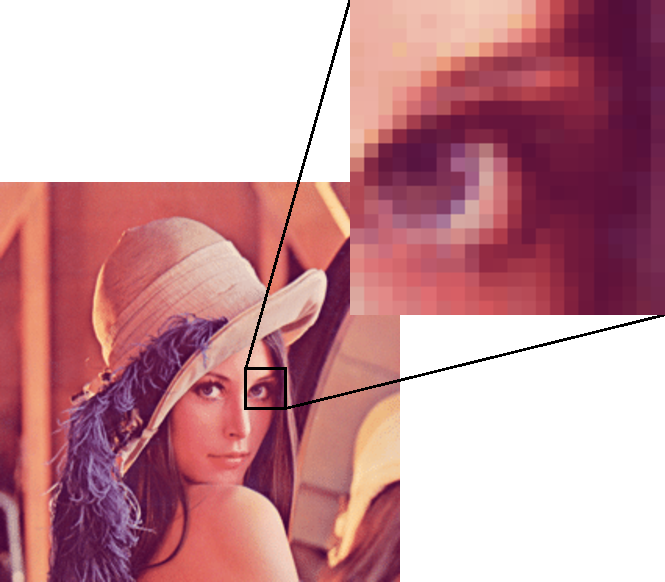
\includegraphics[width=0.5\textwidth]{images/lenaeye.pdf}
  \caption{Lena - detalhe.}\label{fig-lena-detalhe}
  \end{figure}

\end{frame} 

\begin{frame}%[allowframebreaks]
  \frametitle{Espaço necessário para armazenar uma foto}
  \begin{itemize}
  \item câmera 10 Mpixel
  \item 3 bytes por pixel (RGB)
  \item cada foto requer 30 Mbyte
  \item um cartão de memória de 2 Gbytes é capaz de armazenar 66 fotos
  \end{itemize}
\end{frame}

\begin{frame}%[allowframebreaks]
  \frametitle{Espaço necessário para armazenar um vídeo}
  \begin{itemize}
  \item 480 x 720, 30 fps
  \item 345.600 pixels por frame
  \item RGB 3 bytes por pixel
  \item 1.036.800 byte, aprox. 1 Mbyte por frame
  \item 30 frames requerem 31.104.000 bytes, aprox. 31 Mbyte por segundo
  \item um CD de 650 Mbytes é capaz de armazenar apenas 21 segundos de vídeo
  e um DVD de 4.7 GB apenas 155 segundos de vídeo.
  \end{itemize}
\end{frame}


\begin{frame}%[allowframebreaks]
  \frametitle{Dilema de compressão}
  Quando devemos parar a busca por uma \textbf{melhor} compressão?

  \vspace{1cm}
  melhor:
  \begin{itemize}
  \item menor tamanho da representação digital resultante
  \item eficiência computacional (compressão e/ou descompressão)
  \item simplicidade do algoritmo
  \end{itemize}

  \vspace{1cm}
  Qual é o limite de compressão para um determinado dado?

\end{frame} 
\note{
Modificar um algoritmo para melhorar a taxa de compressão em 1\% pode
acarretar um aumento de 10\% no tempo de execução do algoritmo e
ainda mais sobre a complexidade do programa.
}
\note{
Conjecturas\footnote{Uma conjectura é uma proposição que não é provada, mas acredita-se que seja verdadeira e não foi mostrado o contrário.}.
\vspace{2ex}

  \begin{itemize}
  \item Compressão de dados pode ser interpretada como o processo de remover complexidades (redundâncias)
  desnecessárias na informação, e desta forma, maximizando a simplicidade enquanto preserva o máximo
  possível do poder discricionário dos dados.
  \item Todo tipo de computação e racionalização formal pode ser compreendida como compressão
  de informação através do processo de identificar padrões, busca e unificação
  das instâncias destes padrões.
  \end{itemize}

}


\begin{frame}[allowframebreaks]
  \frametitle{Termos}
  \begin{description}
  \item[compressor ou codificador] é o programa que comprime os dados crus na entrada e cria uma saída de dados
  comprimida (com baixa redundância).
  \item[decompressor ou decodificador] converte os dados na direção oposta.
  \item[fluxo] é o dado a ser comprimido, armazenado como um arquivo ou transmitido.
  \item[dado não-codificado, cru, ou original] é o fluxo de dados da entrada.
  \item[dado codificado ou comprimido] é o fluxo de saída.
  \item[método de compressão não-adaptativo] é rígido e não modifica sua operação ou seus parâmetros em resposta
  aos dados em particular que estão sendo comprimidos.
  \item[método adaptativo] analisa os dados crus e modifica sua operação e/ou parâmetros de acordo com os dados em mãos.
  \item[método semi-adaptativo] utiliza 2 passagens aonde, na primeira, realiza a leitura dos dados e
  contabiliza estatísticas dos dados a serem comprimidos; na segunda passagem, realiza de fato a compressão
  utilizados parâmetros determinados na primeira varredura.
  \item[método localmente adaptativo] se adapta às condições locais do fluxo de dados e varia à medida que
  move ao longo dos dados.
  \item[compressão com perdas/sem perdas] : Para atingirem maior compressão, os métodos de compressão com perda
  perdem informação. Os métodos de compressão sem perda não admitem perder informação alguma.
  \item[Compressão em cascata] ocorre quando diferentes métodos de compressão são utilizados um em seguida do outro.
  \item[Compressçao perceptiva] ocorre quando apenas a informação imperceptível pelos nosso sentidos é removida.
  \item[Compressão simétrica] é o caso em que o compressor e descompressor utilizam basicamente o mesmo algoritmo,
  porém em direções opostas.
  \item[Complacente] é o codificador/decodificador que gera/lê de forma correta um fluxo de dados (Qualquer pessoa
  é livre para implementar seu próprio algoritmo).
  \item[Universal] é o método de compressão de dados que não depende da estatística dos dados.
  \item[Razão de Compresão] $=$ tamanho do dado de saída / tamanho do dado de entrada.
  \item[Fator de Compressão] $=$ tamanho do dado de entrada / tamanho do dado de saída $=$ (razão de compressão)$^{-1}$.
  \item[Ganho de Compressão] $= 100 \log_e $ (tamanho de referência / tamanho comprimido), aonde o tamanho de referência é o tamanho dos dados de entrada ou o tamanho do dado de saída comprimido por algum algoritmo padrão.
  \item[Erro médio quadrático (MSE) e relação sinal ruído de sinal (PSNR)] são utilizados para medir a distorção causada por uma compressão com perdas.
  \end{description}
\end{frame} 


\begin{frame}%[allowframebreaks]
  \frametitle{Termos}
  \begin{figure}[h]
  \centering
  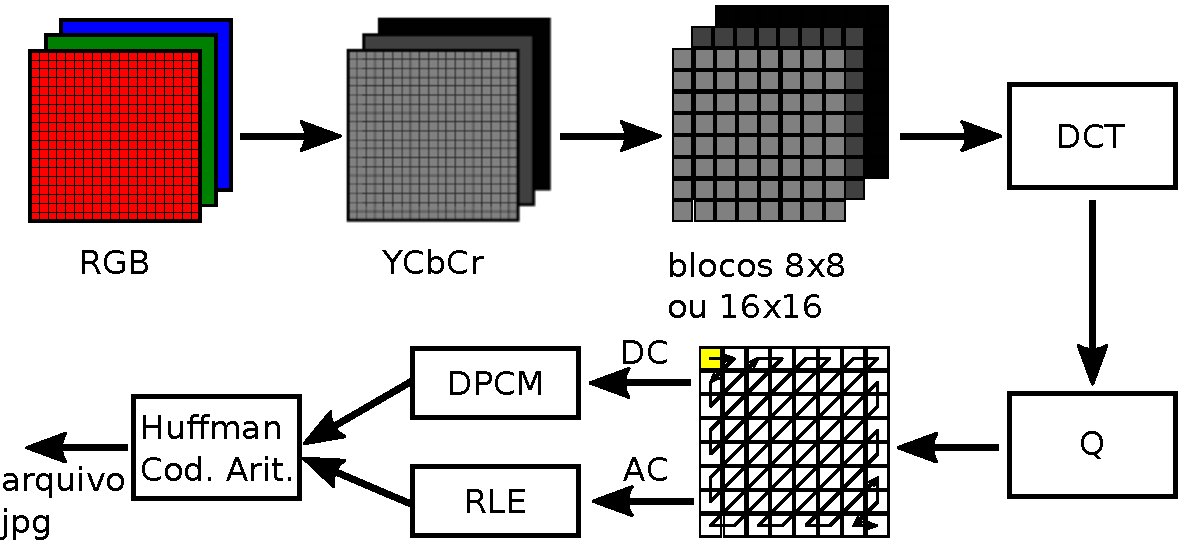
\includegraphics[width=0.8\textwidth]{images/jpegstd.pdf}
  \caption{Esquema de compressão JPEG.}\label{fig-jpegstd}
  \end{figure}
\end{frame} 

\begin{frame}%[allowframebreaks]
  \frametitle{Slides- introdução ao GNU Octave}
  \centering
  
\includegraphics[width=0.4\textwidth]{images/qrcode-octave-intro.pdf}

  \url{https://drive.google.com/open?id=1ew5fl9v_OIybsy3KdEgIvohLTcuwuru_}
\end{frame} 

\begin{frame}%[allowframebreaks]
  \frametitle{Notebook - introdução}
  \centering
  
\includegraphics[width=0.4\textwidth]{images/qrcode-jupyter-intro.pdf}

  \url{https://nbviewer.jupyter.org/github/leolca/notebooks/blob/master/aev/introducao.ipynb}
\end{frame} 

\begin{frame}%[allowframebreaks]
  \frametitle{Notebook - imagem colorida}
  \centering
  
\includegraphics[width=0.4\textwidth]{images/qrcode-jupyter-im-color.pdf}

  \url{https://nbviewer.jupyter.org/github/leolca/notebooks/blob/master/aev/introdocao_imagem_colorida.ipynb}
\end{frame} 



\subsection{Informação}
\begin{frame}%[allowframebreaks]
  \frametitle{Informação}
  O conceito de informação é amplo, sendo difícil ser contemplado em sua plenitude por qualquer definição.

  \vspace{2ex}
  \citet{shannon1948} propôs a definição de \textit{entropia} que possui
  muitas propriedades em comum o senso comum do que deve ser informação.

  \vspace{2ex}
  A informação fornecida por uma mensagem corresponde com o quão improvável é esta mensagem.

\end{frame}
\note{
O que é previsível fornece pouca ou nenhuma informação.

Quanto mais incerto, mais informação há.
}

\begin{frame}%[allowframebreaks]
  \frametitle{Informação}
  \citet{hartley1928} propõem uma medida de informação para uma variável aleatória $X$:
  \begin{equation}
    I(X) = \log_b L ,
  \end{equation}
  onde $L$ é o número de possíveis valores que $X$ pode assumir.
  Se $b=2$, a informação será medida em `bits' (nome sugerido por J.W. Tukey).
\end{frame}
\note{
  A definição de Hartley é condizente com as seguintes intuições sobre informação: 
  \begin{itemize}
  \item Dois cartões de memória devem possuir o dobro da capacidade de um cartão para
  armazenamento de informação.
  \item Dois canais de comunicação idênticos devem possuir o dobro da capacidade 
  de transmitir informação que um único canal.
  \item Um dispositivo com duas posições estáveis, como um relé ou um flip-flop,
  armazena um bit de informação. $N$ dispositivos deste tipo podem armazenar $N$ bits
  de informação, já que o número total de estados é $2^N$ e $\log_2 2^N = N$.
  \end{itemize}

  Entretanto, isto é válido apenas quando as mensagens/eventos são equiprováveis. 
  No caso extremo, note que se o cartão de memória armazena apenas zeros, ele não
  é capaz de armazenar informação alguma.
}

\begin{frame}%[allowframebreaks]
  \frametitle{Entropia}
  Suponha que existam eventos $E_k$ com probabilidade de ocorrência $p_k$. 

  \begin{itemize}
  \item Shannon: informação associada ao evento $E_k$ é dada por $I(E_k) = \log (1/p_k)$.
        \begin{itemize}
        \item Se $p_k=1$ $\rightarrow$ não há surpresa na ocorrência do evento $E_k$.
        \item Se $p_k=0$ $\rightarrow$ surpresa infinita, afinal o evento $E_k$ é impossível.
        \item $I(E_k) = - \log p(E_k)$ é a auto-informação do evento ou mensagem $E_k$.
        \end{itemize}
  \item \textbf{Sempre} utilizaremos a base $2$ para o cálculo do logaritmo, desta forma
  $\log \equiv \log_2$, a menos que seja especificado o contrário.
  \item $\ln$ é o logaritmo na base natural $e$.
  \end{itemize}
\end{frame}

\begin{frame}%[allowframebreaks]
  \frametitle{Entropia}
  \begin{itemize}
  \item Notação: $p(x) = P_X(X=x)$, a probabilidade do evento $\{X=x\}$, da v.a. $X$ assumir o valor $x$.
  \item Valor esperado da v.a. $X$: $E[X] = EX = \sum_x x p(x)$.
  \item Dada uma função $g: \mathcal{X} \rightarrow \mathbb{R}$, o valor esperado da
  v.a. $g(X)$ é $E g(X) = \sum_x g(x) p(x)$.
  \item Considere $g(x) = \log(1/p(x))$. Então $g(x)$ é a imprevisão (surpresa) de encontrar o evento $X=x$.
        Tomando o valor esperado de $g$ teremos
        \begin{equation}
        \sum_x p(x) \log \frac{1}{p(x)} ,
        \end{equation}
        ou seja, a esperança da surpresa, ou o valor esperado da imprevisão na variável aleatória $X$.
        Esta é a definição de entropia.
  \end{itemize}
\end{frame}


% entropia
\section{Entropia}
\subsection{Definição de entropia}
\begin{frame}%[allowframebreaks]
  \frametitle{Entropia}
  \begin{definition}[Entropia]\label{def-entropia}
  Dada uma variável aleatória $X$ sob um alfabeto de tamanho finito $\mathcal{X}$, a \textbf{entropia}
  da variável aleatória é dada por
  \begin{eqnarray}
  H(X) &\triangleq& E_p \log \frac{1}{p(X)} = E \log \frac{1}{p(X)} \\
        &=& \sum_{x \in \mathcal{X}} p(x) \log \frac{1}{p(x)} = - \sum_x p(x) \log p(x)
  \end{eqnarray}
  \end{definition}
  A unidade de entropia é `bits', já que utilizamos o logaritmo na base $2$ (unidade `nats' se 
  utilizar a base $e$).
\end{frame}
\note{  
  \begin{itemize}
  \item Entropia mede a grau de incerteza associado a uma distribuição.
  \item Entropia mede a desordem ou o espalhamento de uma distribuição.
  \item Entropia mede a `escolha' que a fonte tem na escolha de símbolos de acordo com uma densidade 
        (maior entropia implica em mais escolha).
  \item Vamos utilizar a seguinte convenção: $0 \log 0 = 0$.
  \end{itemize}
}

\begin{frame}%[allowframebreaks]
  \frametitle{Entropia}
  Se uma v.a. $X \sim p(x)$, então o valor esperado de uma função desta v.a., $g(X)$, é dada por
  \begin{equation}
  E[g(X)] = \sum_{x \in \mathcal{X}} p(x) g(x) .
  \end{equation}

  A entropia de $X$ pode ser interpretada como o valor esperado da v.a. $\log \frac{1}{p(X)}$,
  onde $X$ é descrita pela função massa de probabilidade $p(x)$.
  \begin{equation}
  H(X) = E \left[ \log \frac{1}{p(X)} \right] .
  \end{equation}
\end{frame}
\note{
  \begin{itemize}
  \item Entropia é uma medida da real `incerteza' média, o que é uma medida sobre toda a distribuição.
  \item Entropia mede o grau de incerteza médio ou esperado do resultado de uma distribuição de probabilidade.
  \item É uma medida de desordem ou espalhamento. Distribuições com alta entropia devem ser planas, mais
  uniformes, enquanto distribuições com baixa entropia devem possuir poucas modas (unimodal, bimodal).
  \end{itemize}
}
\note{
  \begin{figure}[h!]
  \centering
  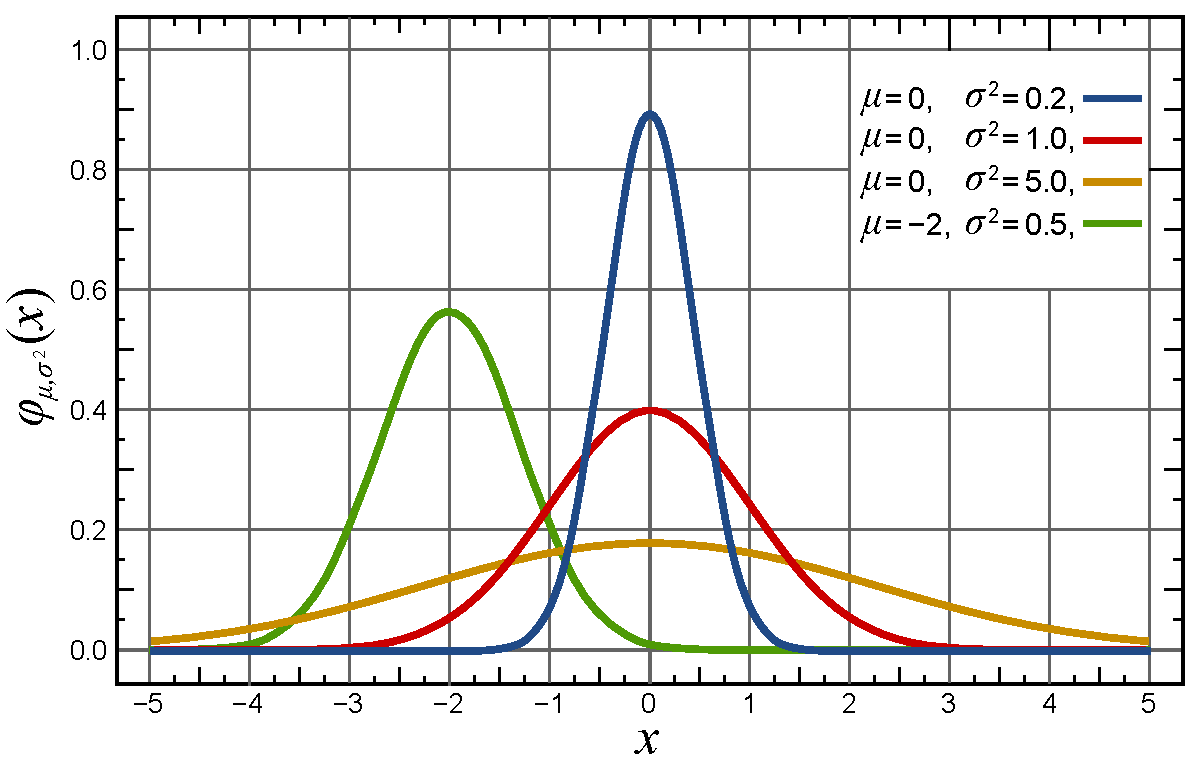
\includegraphics[width=0.4\textwidth]{images/normal_distribution.pdf}
  %\caption{.}
  \label{fig:normal_distribution}
  \end{figure}

  \begin{itemize}
  \item mais concentrado: menor entropia
  \item mais espalhado: maior entropia
  \item os valores em $x$ não importam, 
  apenas os valores das probabilidades associadas $p(x)$ importam no cálculo da entropia
  \end{itemize}
}

\begin{frame}[allowframebreaks]
  \frametitle{Escolha, Incerteza e Entropia}
  Suponha um conjunto de eventos cujas probabilidades de ocorrências sejam dadas
  por $p_1, p_2, \ldots, p_n$. É possível encontrar uma medida de quanta `escolha' 
  está envolvida na seleção de um evento ou quão incertos estamos da saída?

  Para tal medida $H(p_1, p_2, \ldots, p_n)$, é razoável requerermos as seguintes propriedades:
  \begin{enumerate}
  \item $H$ deve ser contínuo em $p_i$;
  \item Se todos os $p_i$ são iguais, $p_i=\frac{1}{n}$, então $H$ deve ser uma função
  monotonicamente crescente de $n$ (quando temos eventos equiprováveis, teremos mais incerteza
  quão maior for o número de eventos possíveis);
  \item Se for possível quebrar uma escolha em uma sequência de escolhas sucessivas,
  a medida $H$ original deve ser a soma ponderada dos valores individuais das medidas
  $H_i$ após a quebra.
  
     \begin{figure}[h!]
     \centering
     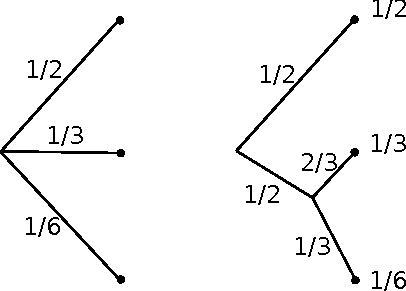
\includegraphics[width=0.3\textwidth]{images/entr-quebra.pdf}
     %\caption{Df.}
     \label{fig:entr-quebra}
     \end{figure}

  \begin{equation}
  H(\frac{1}{2},\frac{1}{3},\frac{1}{6}) = H(\frac{1}{2},\frac{1}{2}) + \frac{1}{2} H(\frac{2}{3},\frac{1}{3})
  \end{equation}
  \end{enumerate}

  A única função $H$ que satisfaz às suposições acima é da forma \cite{shannon1948}: 
  \begin{equation}\label{eq-K-entropia}
  H = - K \sum_{i=1}^{k} p(i) \log p(i) \textmd{ ,}
  \end{equation} 
  onde $K$ é uma constante positiva. 
\end{frame}




\subsection{Demonstração da equação da entropia}
\begin{frame}[allowframebreaks]
  \frametitle{Demonstração da \Cref{eq-K-entropia}}

  Nesta secção iremos apresentar a demonstração de $H=-\sum p_i \log p_i$ 
  (conforme Apêndice 2 de \citet{shannon1948}).

  Vamos definir
  \begin{equation}
  A(n) = H\left( \frac{1}{n}, \frac{1}{n}, \ldots, \frac{1}{n} \right) .
  \end{equation}

  Desejamos que uma escolha dentre $s^m$ opções igualmente prováveis possa ser decomposta como uma sequência de $m$ escolhas
  que se subdividem em $s$ possibilidades igualmente prováveis.

  \begin{figure}[h!]
  \centering
  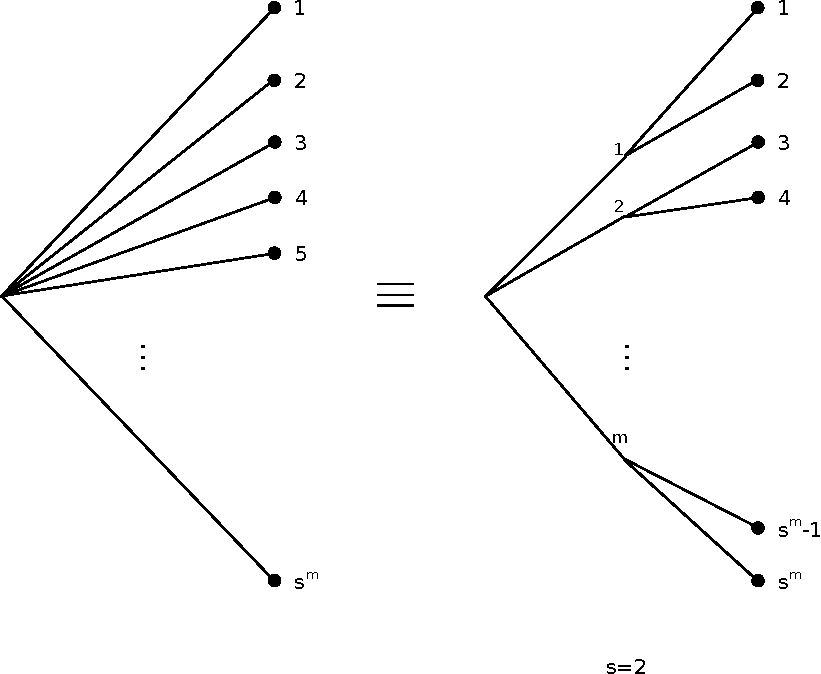
\includegraphics[width=0.5\textwidth]{images/choices.pdf}
  \caption{Exemplo de equivalência para $s=2$.}
  \label{fig:choiceseqv}
  \end{figure}

  Teremos então que
  \begin{equation}
  A(s^m) = m A(s) .
  \end{equation}
  Da mesma forma, para $t$ e $n$, teremos $A(t^n) = n A(t)$.
  Podemos tomar $n$ arbitrariamente grande e encontrar $m$ que satisfaça
  \begin{equation}
  s^m \leq t^n \leq s^{(m+1)} .
  \end{equation}
  Tomando o logaritmo\footnote{Logaritmo é uma função monótona crescente.} da expressão acima e dividindo 
  por $n \log s$ todos os termos\footnote{$n \log s$ é positivo para $n \geq 0$ e $s \geq 1$.}, teremos
  \begin{equation}
  \frac{m}{n} \leq \frac{\log t}{\log s} \leq \frac{m}{n} + \frac{1}{n} ,
  \end{equation}
  o que é equivalente a 
  \begin{equation}
  \left\vert \frac{m}{n} - \frac{\log t}{\log s} \right\vert < \epsilon ,
  \end{equation}
  onde $\epsilon$ é arbitrariamente pequeno, já que $n$ é arbitrariamente grande.

  Usando agora a propriedade desejada de monotonicidade de $A(n)$, teremos
  \begin{alignat}{3}
  A(s^m) &\leq A(t^n) &\leq A(s^{(m+1)}) \nonumber \\
  mA(s) &\leq nA(t) &\leq (m+1)A(s)
  \end{alignat}

  Dividindo a expressão acima por $nA(s)$, teremos
  \begin{equation}
  \frac{m}{n} \leq \frac{A(t)}{A(s)} \leq \frac{m}{n} + \frac{1}{n} ,
  \end{equation}
  ou, de forma equivalente,
  \begin{equation}
  \left\vert \frac{m}{n} - \frac{A(t)}{A(s)} \right\vert < \epsilon ,
  \end{equation}
  e assim, como as duas frações ($\nicefrac{\log t}{\log s}$ e $\nicefrac{A(t)}{A(s)}$) estão $\epsilon$ próximas
  de $\nicefrac{m}{n}$, podemos concluir que
  \begin{equation}
  \left\vert \frac{A(t)}{A(s)} - \frac{\log t}{\log s} \right\vert < 2\epsilon .
  \end{equation}
  Como $\epsilon$ é arbitrariamente pequeno, no limite teremos
  \begin{eqnarray}
  \frac{A(t)}{A(s)} &=& \frac{\log t}{\log s} \nonumber \\
  A(t) &=& \frac{A(s)}{\log s} \log t = K \log t ,
  \end{eqnarray}
  onde $K$ deve ser positivo, de forma que $A(n)$ seja monótona crescente.

  Suponha uma escolha com $n$ possibilidades em que as probabilidades são comensuráveis,
  $p_i = \nicefrac{n_i}{\sum n_i}$, onde $n_i$ são inteiros. De forma equivalente,
  uma escolha entre $\sum n_i$ opções pode ser expressa como uma escolha dentre $n$ opções
  com probabilidades $p_1, \ldots, p_n$, e para uma $i$-ésima dada escolha, realizar uma
  nova escolha dentre $n_i$ opções igualmente prováveis. Teremos então:
  \begin{eqnarray}
  \overbrace{ K \log \left( \sum n_i \right) }^{A\left( \sum n_i \right)} &=& H(p_1, \ldots, p_n) + \overbrace{ K \log n_i }^{A(n_i)} \nonumber \\
  K \underbrace{\left( \sum p_i \right)}_{=1} \log \left( \sum n_i \right) &=& H(p_1, \ldots, p_n) + K \underbrace{\left( \sum p_i \right)}_{=1} \log n_i .
  \end{eqnarray}  
  E assim,
  \begin{eqnarray}
  H(p_1, \ldots, p_n) &=& K\left[ \left( \sum p_i \right) \log \left( \sum n_i \right) - \left( \sum p_i \right) \log n_i \right] \nonumber \\
        &=& -K \sum p_i \log \frac{n_i}{\sum n_i} = -K \sum p_i \log p_i . \qed
  \end{eqnarray} 
\end{frame}



\subsection{Entropia - Fonte Binária}
\begin{frame}%[allowframebreaks]
  \frametitle{Entropia Binária}
  \begin{itemize}
  \item Alfabeto binário $X \in \{0,1\}$, ou $\mathcal{X} = \{0,1\}$.
  \item $p(X=1)=p=1-p(X=0)$.
  \item $H(X) = -p \log p - (1-p) \log (1-p) = H(p)$.
  \item entropia como função de $p$

  \begin{figure}[h!]
  \centering
  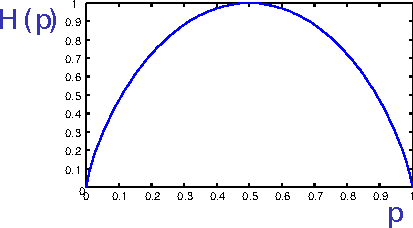
\includegraphics[width=0.5\textwidth]{images/graph_Hp.pdf}
  %\caption{.}
  \label{fig:graph_Hp}
  \end{figure}
  \end{itemize}
\end{frame}
\note{
  \begin{itemize}
  \item maior incerteza ($H=1$) quando $p=0.5$ e menor incerteza ($H=0$) quando $p=0$ ou $p=1$.
  \item note que a entropia $H(p)$ é concava em $p$.
  \end{itemize}
}


\begin{frame}%[allowframebreaks]
  \frametitle{Entropia - GNU Octave}
  \lstinputlisting[firstline=30,lastline=41,label=lst-entropy-fnc]{/home/leoca/ee/research/clscripts/entropy.m}

  \href{https://raw.githubusercontent.com/leolca/clscripts/master/entropy.m}{[download do código]}
\end{frame}

\begin{frame}%[allowframebreaks]
  \frametitle{Entropia - GNU Octave - demo}
  \lstinputlisting[firstline=43,lastline=51,label=lst-entropy-fnc]{/home/leoca/ee/research/clscripts/entropy.m}
\end{frame}






\bibliographystyle{apalike}
\bibliography{bibliografia}
\label{bibliografia}

\end{document}

